\documentclass[12pt]{article}

% packages
\usepackage{kantlipsum}
\usepackage[margin=1in]{geometry}
\usepackage[labelfont=it]{caption}
\usepackage[table]{xcolor}
\usepackage{subcaption,framed,colortbl,multirow}
\usepackage{amsmath,amsthm,amssymb,wasysym,mathrsfs,mathtools}
\usepackage{tikz,graphicx,pgf,pgfplots}
\usetikzlibrary{arrows, angles, quotes, decorations.pathreplacing, math, patterns, calc}
\pgfplotsset{compat=1.16}

% custom commands
\newcommand{\N}{\mathbb{N}}
\newcommand{\Z}{\mathbb{Z}}
\newcommand{\I}{\mathbb{I}}
\newcommand{\R}{\mathbb{R}}
\newcommand{\Q}{\mathbb{Q}}
\newcommand{\C}{\mathbb{C}}
\newcommand{\F}{\mathbb{F}}
\newcommand{\p}{^{\prime}}
\newcommand{\powerset}{\raisebox{.15\baselineskip}{\Large\ensuremath{\wp}}}
\DeclarePairedDelimiter{\ceil}{\lceil}{\rceil}
\DeclarePairedDelimiter\floor{\lfloor}{\rfloor}

\setlength{\fboxsep}{4pt}
\newcommand{\exercise}[2]{\section*{Exercise #1}\begin{center}\framebox{\begin{minipage}{\textwidth-10pt}#2\end{minipage}}\end{center}}
\newcommand{\problem}[2]{\section*{Problem #1}\begin{center}\framebox{\begin{minipage}{\textwidth-10pt}#2\end{minipage}}\end{center}}
\newcommand{\generic}[2]{\section*{#1}\begin{center}\framebox{\begin{minipage}{\textwidth-10pt}#2\end{minipage}}\end{center}}

 
\begin{document}
 
\title{Homework 4\\
    \large MATH CS 120CT Category Theory}
\author{Harry Coleman}
\date{January 29, 2020}
\maketitle


\exercise{1}{
    How many functors are there from \textbf{2} to \textbf{3}? How many natural transformations are there amongst these functors?
}

Shown in figure \ref{fig:cats} are the given categories.

\begin{figure}[ht]
    \centering
    \begin{subfigure}[b]{.47\textwidth}
        \centering
        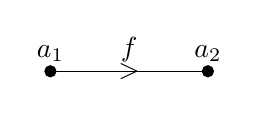
\begin{tikzpicture}
            \draw[fill=black] (0,0) circle (2pt) node[anchor=south]{$a_1$};
            \draw[fill=black] (2,0) circle (2pt) node[anchor=south]{$a_2$};
            
            \draw[] (0,0) -- (2,0) node[midway]{$>$} node[midway, anchor=south]{$f$};
        \end{tikzpicture}
        \caption{The free category \textbf{2}}
        \label{fig:cat1}
    \end{subfigure}
    \begin{subfigure}[b]{.47\textwidth}
        \centering
        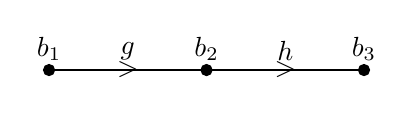
\begin{tikzpicture}
            \draw[fill=black] (0,0) circle (2pt) node[anchor=south]{$b_1$};
            \draw[fill=black] (2,0) circle (2pt) node[anchor=south]{$b_2$};
            \draw[fill=black] (4,0) circle (2pt) node[anchor=south]{$b_3$};
            
            \draw[] (0,0) -- (2,0) node[midway]{$>$} node[midway, anchor=south]{$g$};
            \draw[] (2,0) -- (4,0) node[midway]{$>$} node[midway, anchor=south]{$h$};
        \end{tikzpicture}
        \caption{The free category \textbf{3}}
        \label{fig:cat2}
    \end{subfigure}
    \caption{}
    \label{fig:cats}
\end{figure}

From these, we find 6 possible functors from \textbf{2} to \textbf{3}, which are
\begin{alignat*}{4}
    F: &\quad& a_1 \mapsto b_1,  &\quad& a_2 \mapsto b_1, &\quad f\mapsto id_{b_1};& \\
    G: &\quad& a_1 \mapsto b_1,  &\quad& a_2 \mapsto b_2, &\quad f\mapsto g;& \\
    H: &\quad& a_1 \mapsto b_1,  &\quad& a_2 \mapsto b_3, &\quad f\mapsto h\circ g;& \\
    I: &\quad& a_1 \mapsto b_2,  &\quad& a_2 \mapsto b_2, &\quad f\mapsto id_{b_2};& \\
    J: &\quad& a_1 \mapsto b_2,  &\quad& a_2 \mapsto b_3, &\quad f\mapsto h;& \\
    K: &\quad& a_1 \mapsto b_3,  &\quad& a_2 \mapsto b_3, &\quad f\mapsto id_{b_3}.&
\end{alignat*}
There are other possible ways to map objects and morphism from \textbf{2} to \textbf{3}, however, these are the only ones which preserve the structure of $f$, the one morphism in \textbf{2}.

To find a natural transformation $\alpha$ between two functors $X,Y:\textbf{2}\rightarrow\textbf{3}$, we must find assignments of objects in \textbf{2} to morphisms in \textbf{3} which satisfy the commutative diagram in figure \ref{fig:square}.

\begin{figure}[ht]
    \centering
    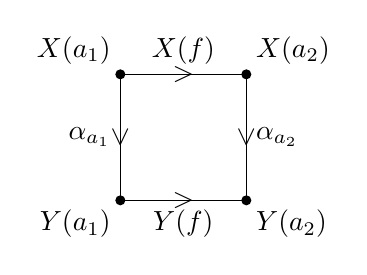
\begin{tikzpicture}[scale=0.8]
        \draw[fill=black] (0,2) circle (2pt) node[anchor=south east]{$X(a_1)$};
        \draw[fill=black] (2,2) circle (2pt) node[anchor=south west]{$X(a_2)$};
        \draw[fill=black] (0,0) circle (2pt) node[anchor=north east]{$Y(a_1)$};
        \draw[fill=black] (2,0) circle (2pt) node[anchor=north west]{$Y(a_2)$};
        
        \draw[] (0,2) -- (2,2) node[midway]{$>$} node[midway, anchor=south]{$X(f)$};
        \draw[] (0,0) -- (2,0) node[midway]{$>$} node[midway, anchor=north]{$Y(f)$};
        \draw[] (0,2) -- (0,0) node[midway, rotate=-90]{$>$} node[midway, anchor=east]{$\alpha_{a_1}$};
        \draw[] (2,2) -- (2,0) node[midway, rotate=-90]{$>$} node[midway, anchor=west]{$\alpha_{a_2}$};
    \end{tikzpicture}
    \caption{Commutative diagram for natural transformations between functors from \textbf{2} to \textbf{3}.}
    \label{fig:square}
\end{figure}



With this, we find 20 possible natural transformations, which are
\begin{alignat*}{4}
    \alpha^1: &\quad& F&\rightarrow F, \quad& \alpha^1_{a_1}= &id_{b_1}, \quad& \alpha^1_{a_2}= &id_{b_1} ; \\
    \alpha^2: &\quad& F&\rightarrow G, \quad& \alpha^2_{a_1}= &id_{b_1}, \quad& \alpha^2_{a_2}= &g ; \\
    \alpha^3: &\quad& F&\rightarrow H, \quad& \alpha^3_{a_1}= &id_{b_1}, \quad& \alpha^3_{a_2}= &h\circ g ; \\
    \alpha^4: &\quad& F&\rightarrow I, \quad& \alpha^4_{a_1}= &g, \quad& \alpha^4_{a_2}= &g ; \\
    \alpha^5: &\quad& F&\rightarrow J, \quad& \alpha^5_{a_1}= &g, \quad& \alpha^5_{a_2}= &h\circ g ; \\
    \alpha^6: &\quad& F&\rightarrow K, \quad& \alpha^6_{a_1}= &h\circ g, \quad& \alpha^6_{a_2}= &h\circ g ; \\
    \alpha^7: &\quad& G&\rightarrow G, \quad& \alpha^7_{a_1}= &id_{b_1}, \quad& \alpha^7_{a_2}= &id_{b_2} ; \\
    \alpha^8: &\quad& G&\rightarrow H, \quad& \alpha^8_{a_1}= &id_{b_1}, \quad& \alpha^8_{a_2}= &h ; \\
    \alpha^9: &\quad& G&\rightarrow I, \quad& \alpha^9_{a_1}= &g, \quad& \alpha^9_{a_2}= &id_{b_2} ; \\
    \alpha^{10}: &\quad& G&\rightarrow J, \quad& \alpha^{10}_{a_1}= &g, \quad& \alpha^{10}_{a_2}= &h ; \\
    \alpha^{11}: &\quad& G&\rightarrow K, \quad& \alpha^{11}_{a_1}= &h\circ g, \quad& \alpha^{11}_{a_2}= &h ; \\
    \alpha^{12}: &\quad& H&\rightarrow H, \quad& \alpha^{12}_{a_1}= &id_{b_1}, \quad& \alpha^{12}_{a_2}= &id_{b_3} ; \\
    \alpha^{13}: &\quad& H&\rightarrow J, \quad& \alpha^{13}_{a_1}= &g, \quad& \alpha^{13}_{a_2}= &id_{b_3} ; \\
    \alpha^{14}: &\quad& H&\rightarrow K, \quad& \alpha^{14}_{a_1}= &h\circ g, \quad& \alpha^{14}_{a_2}= &id_{b_3} ; \\
    \alpha^{15}: &\quad& I&\rightarrow I, \quad& \alpha^{15}_{a_1}= &id_{b_2}, \quad& \alpha^{15}_{a_2}= &id_{b_2} ; \\
    \alpha^{16}: &\quad& I&\rightarrow J, \quad& \alpha^{16}_{a_1}= &id_{b_2}, \quad& \alpha^{16}_{a_2}= &h ; \\
    \alpha^{17}: &\quad& I&\rightarrow K, \quad& \alpha^{17}_{a_1}= &h, \quad& \alpha^{17}_{a_2}= &h ; \\
    \alpha^{18}: &\quad& J&\rightarrow J, \quad& \alpha^{18}_{a_1}= &id_{b_2}, \quad& \alpha^{18}_{a_2}= &id_{b_1} ; \\
    \alpha^{19}: &\quad& J&\rightarrow K, \quad& \alpha^{19}_{a_1}= &h, \quad& \alpha^{19}_{a_2}= &id_{b_3} ; \\
    \alpha^{20}: &\quad& K&\rightarrow K, \quad& \alpha^{20}_{a_1}= &id_{b_3}, \quad& \alpha^{20}_{a_2}= &id_{b_3}.
\end{alignat*}

The notion of a component $\alpha_x$ being equal to a particular morphism may not be correct; the symbol $=$ is used to refer to the relation of an object in \textbf{2} to a morphism in \textbf{3}, in the context of a natural transformation. We are also considering the natural transformations from functors to themselves, where components are simply the identity morphisms.

Because \textbf{2} and \textbf{3} have a "one-way" sort of morphism structure, if there is a natural transformation from one functor to another, the natural transformation does not exist in the opposite direction (unless they are the same functor). However, this is not necessarily true in general.






\end{document}